\section{Size of the pilot study.\label{app_ss10}}

\subsection{Pilot study sample size for different screening thresholds}

One of the most important parameters for the applied researcher when performing the power analysis presented in this paper is the size of the pilot study.  Pilot data is expensive and should be kept to a minimum while preserving its power estimation benefit.  However, this method is based on the empirical distribution of the peaks above the screening threshold, which means only effects above this screening threshold can be observed.  For example, when using the default screening threshold from SPM ($p=0.001, t=3.09$),  the effect size in a pilot study with 10 subjects only surpasses the screening threshold with an effect size of Cohen's $d$ of 0.98 ($=3.09/\sqrt{10}$).
The minimally detectable effects for FSL's and SPM's default screening thresholds are presented in Table \ref{mindeteff}.  However, our method estimates the alternative distribution as a truncated normal distribution, and therefore allows a portion of the distribution (and even the mean) to be below the screening threshold.  This fact notwithstanding, it is clear that a very small effect size that hardly surpasses the screening threshold is problematic for this estimation procedure.  In this main body of this paper, we have used a screening threshold, but we present results for the simulations and HCP-validation in the next subsection.

\begin{table}
\begin{center}
\begin{tabular}{lll}
\toprule
& FSL & SPM \\
& ($t=2.3$) & ($p=0.001$) \\
\midrule
5 & 1.03 & 1.38\\
10 & 0.73 & 0.98\\
15 & 0.59 & 0.80\\
20 & 0.51 & 0.69\\
\bottomrule
\end{tabular}
\end{center}
\caption{Given a screening threshold (defaults from popular software are given), how big should the Cohen's D effect be to be observable? \label{mindeteff}}
\end{table}

We show that for a sample size of 10 subjects for small effects, the procedure leads to large overestimation of the power.  The reason is the following: when our procedure predicts that 90\% power will be reached at sample size $n^*$, this means that 90\% of the effects that are large enough to be detectable in the pilot study will become significant with $n^*$ subjects.  As such, our procedure ignores the effects that weren't detectable in the pilot data.  These undetectable effects are by definition small and harder to deem significant with $n^*$ subjects, leading to the observed overestimation in power calculations for a small pilot study sample size.  This effect can be seen both for simulated data and the HCP data.
Another problem that arises with a small pilot study sample size is that the FDR controlling procedure hardly ever finds a threshold in the pilot study, and as such power calculations are almost impossible except for high effect sizes.


\subsection{Results of simulation with pilot sample size of 10 subjects}

Figure \ref{SIM_model_10} and \ref{SIM_pow_10} show the results of the validation procedure for the simulations with a pilot dataset with sample size 10.  The results follow the same patterns of the results with a pilot sample size of 15, but all errors are largely blown up.  That is, the effect size estimation is still problematic when only few activations are present, but this effect remains for very large effects too.  The consequence is a large underestimation for the power calculations in all conditions.  The effect for FDR control, when a pilot study is often impossible due to an estimation of $\pi_1=0$ is repeated in all different conditions, except for very high values of power.

\begin{center}
\begin{figure}[h]
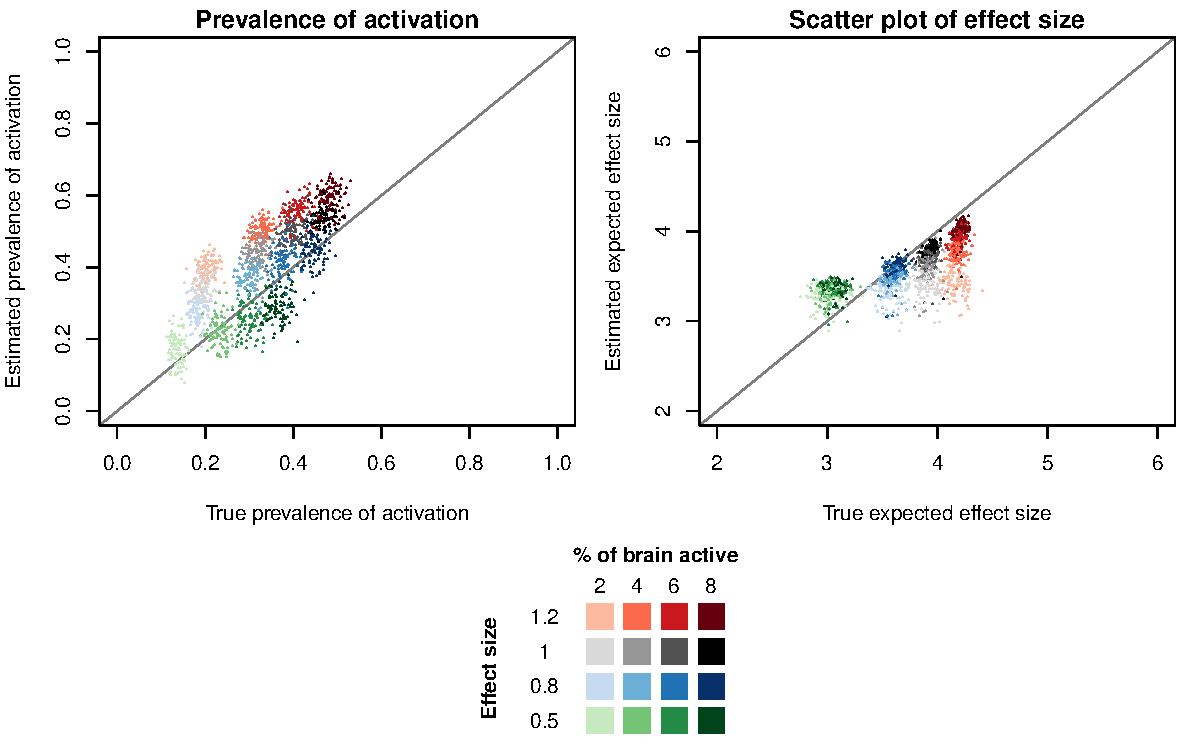
\includegraphics[scale=0.8]{FIG_SIM_modelestimation_10_NOMASK_2_5.pdf}
\caption{Simulation results.  Left: Plot of estimated $\hat\pi_1$ against true $\pi_1$ for different sample sizes and different values for $\mu_1$. Each dot represents a different simulation, as such there are 500 dots for each condition.  Right: Plot of estimated expected peak height $\hat\mu_1$ against true expected peak height $\mu_1$ for different effect sizes. The estimations are the result for a pilot dataset with $n=10$.  \label{SIM_model_10}}
\end{figure}
\end{center}

\begin{center}
\begin{figure}[h]
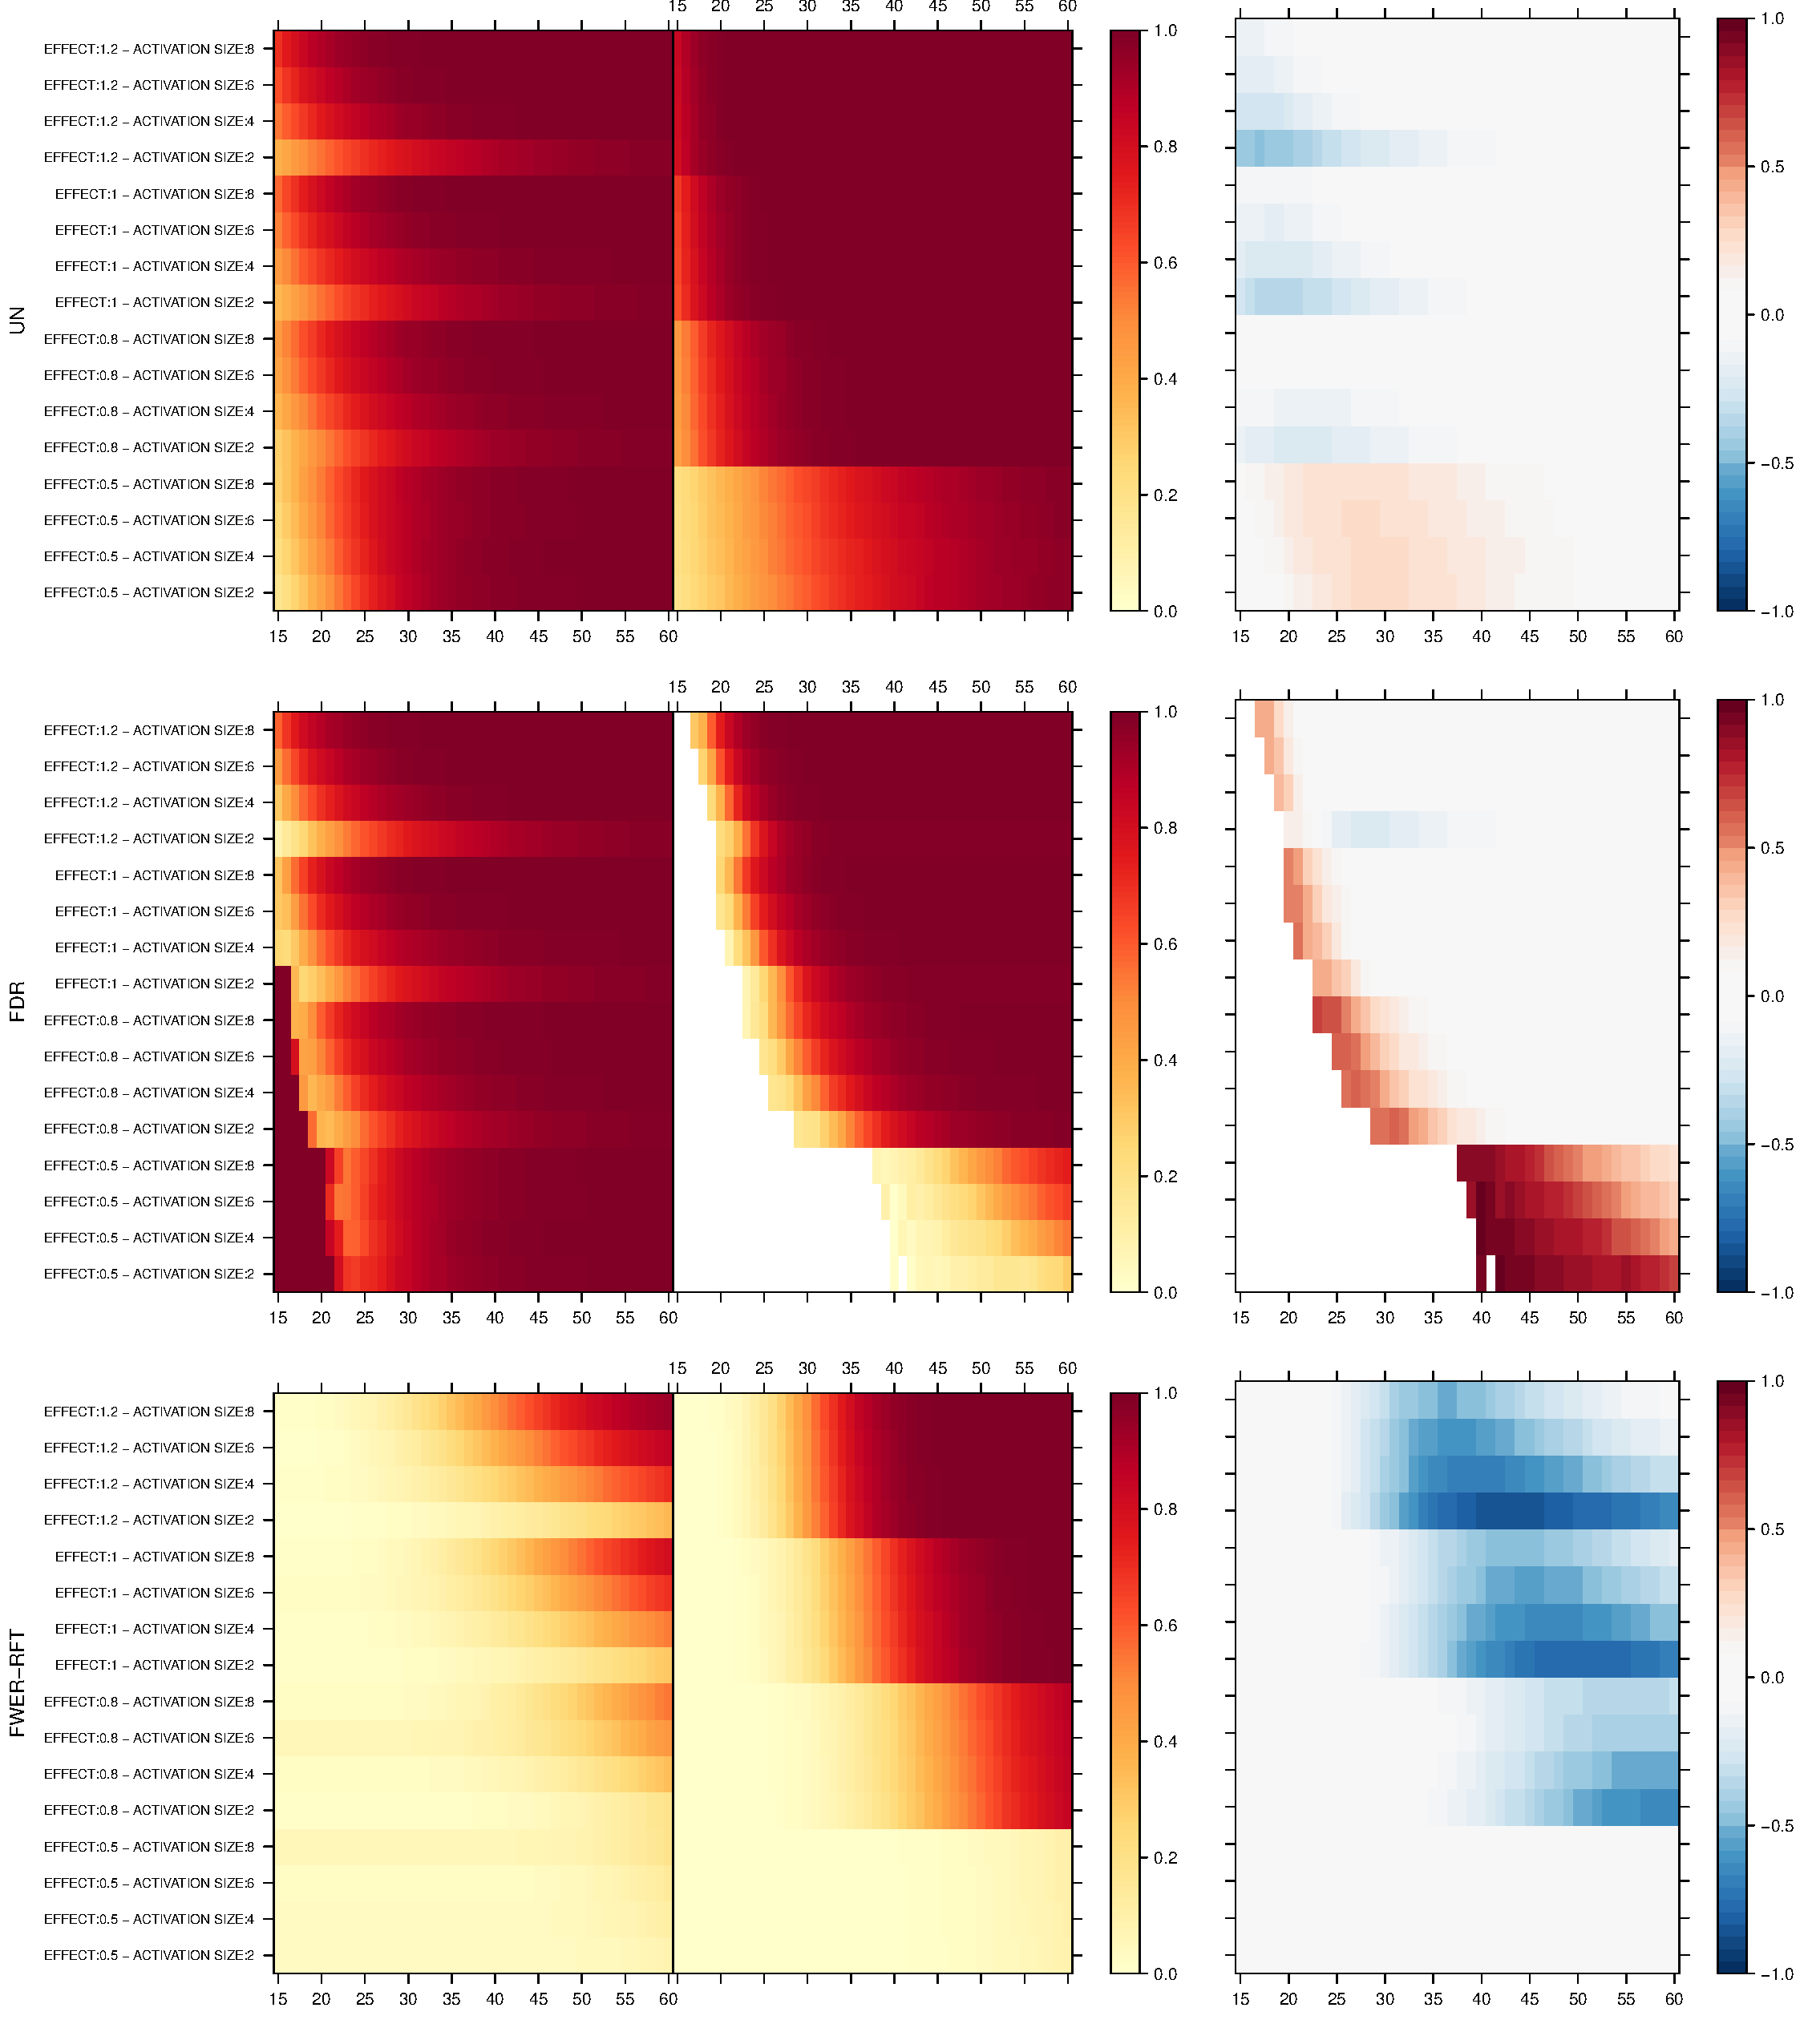
\includegraphics[scale=0.4]{FIG_SIM_power_10_NOMASK_2_5.pdf}
\caption{Simulation results.  Plots of the peakwise average power with error rate control at 5\% for different effect sizes and different amounts of activation.  The left column shows the estimated power curves, the middle column shows the true power and the right column shows the bias.  Bias is defined as the estimated power minus the true power.  The peakwise average power is estimated from a pilot study with 10 subjects. \label{SIM_pow_10}}
\end{figure}
\end{center}

\begin{center}
\begin{figure}[h]
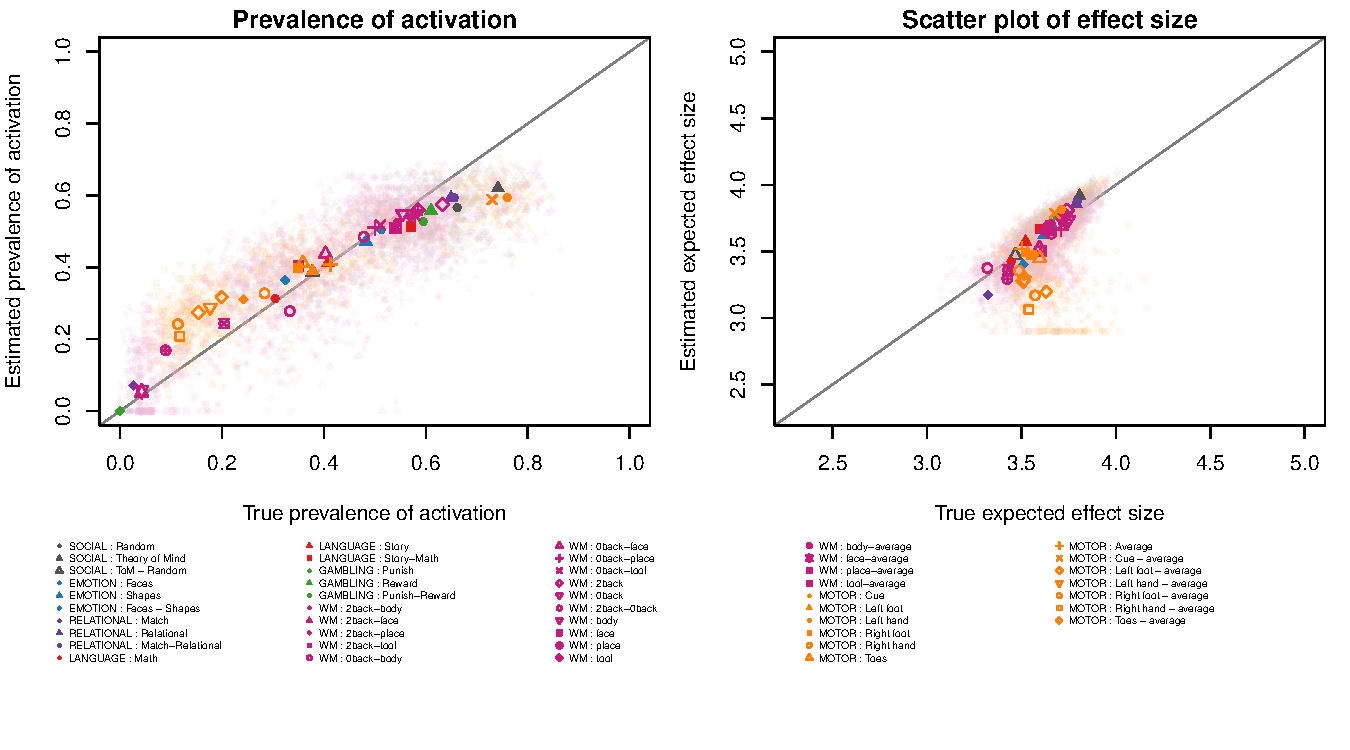
\includegraphics[scale=0.8]{FIG_HCP_10_modelestimation.pdf}
\caption{HCP results.  Left: Plots of estimated $\hat\pi_1$ against true $\pi_1$ for different sample sizes and different values for $\mu_1$. Each dot represents a different simulation, as such there are 500 dots for each condition.  Right: Plot of estimated expected peak height $\hat\mu_1$ against true expected peak height $\mu_1$ for different effect sizes. The estimations are the result for a pilot dataset with $n=10$.  \label{SIM_model_10}}
\end{figure}
\end{center}


\begin{center}
\begin{figure}[h]
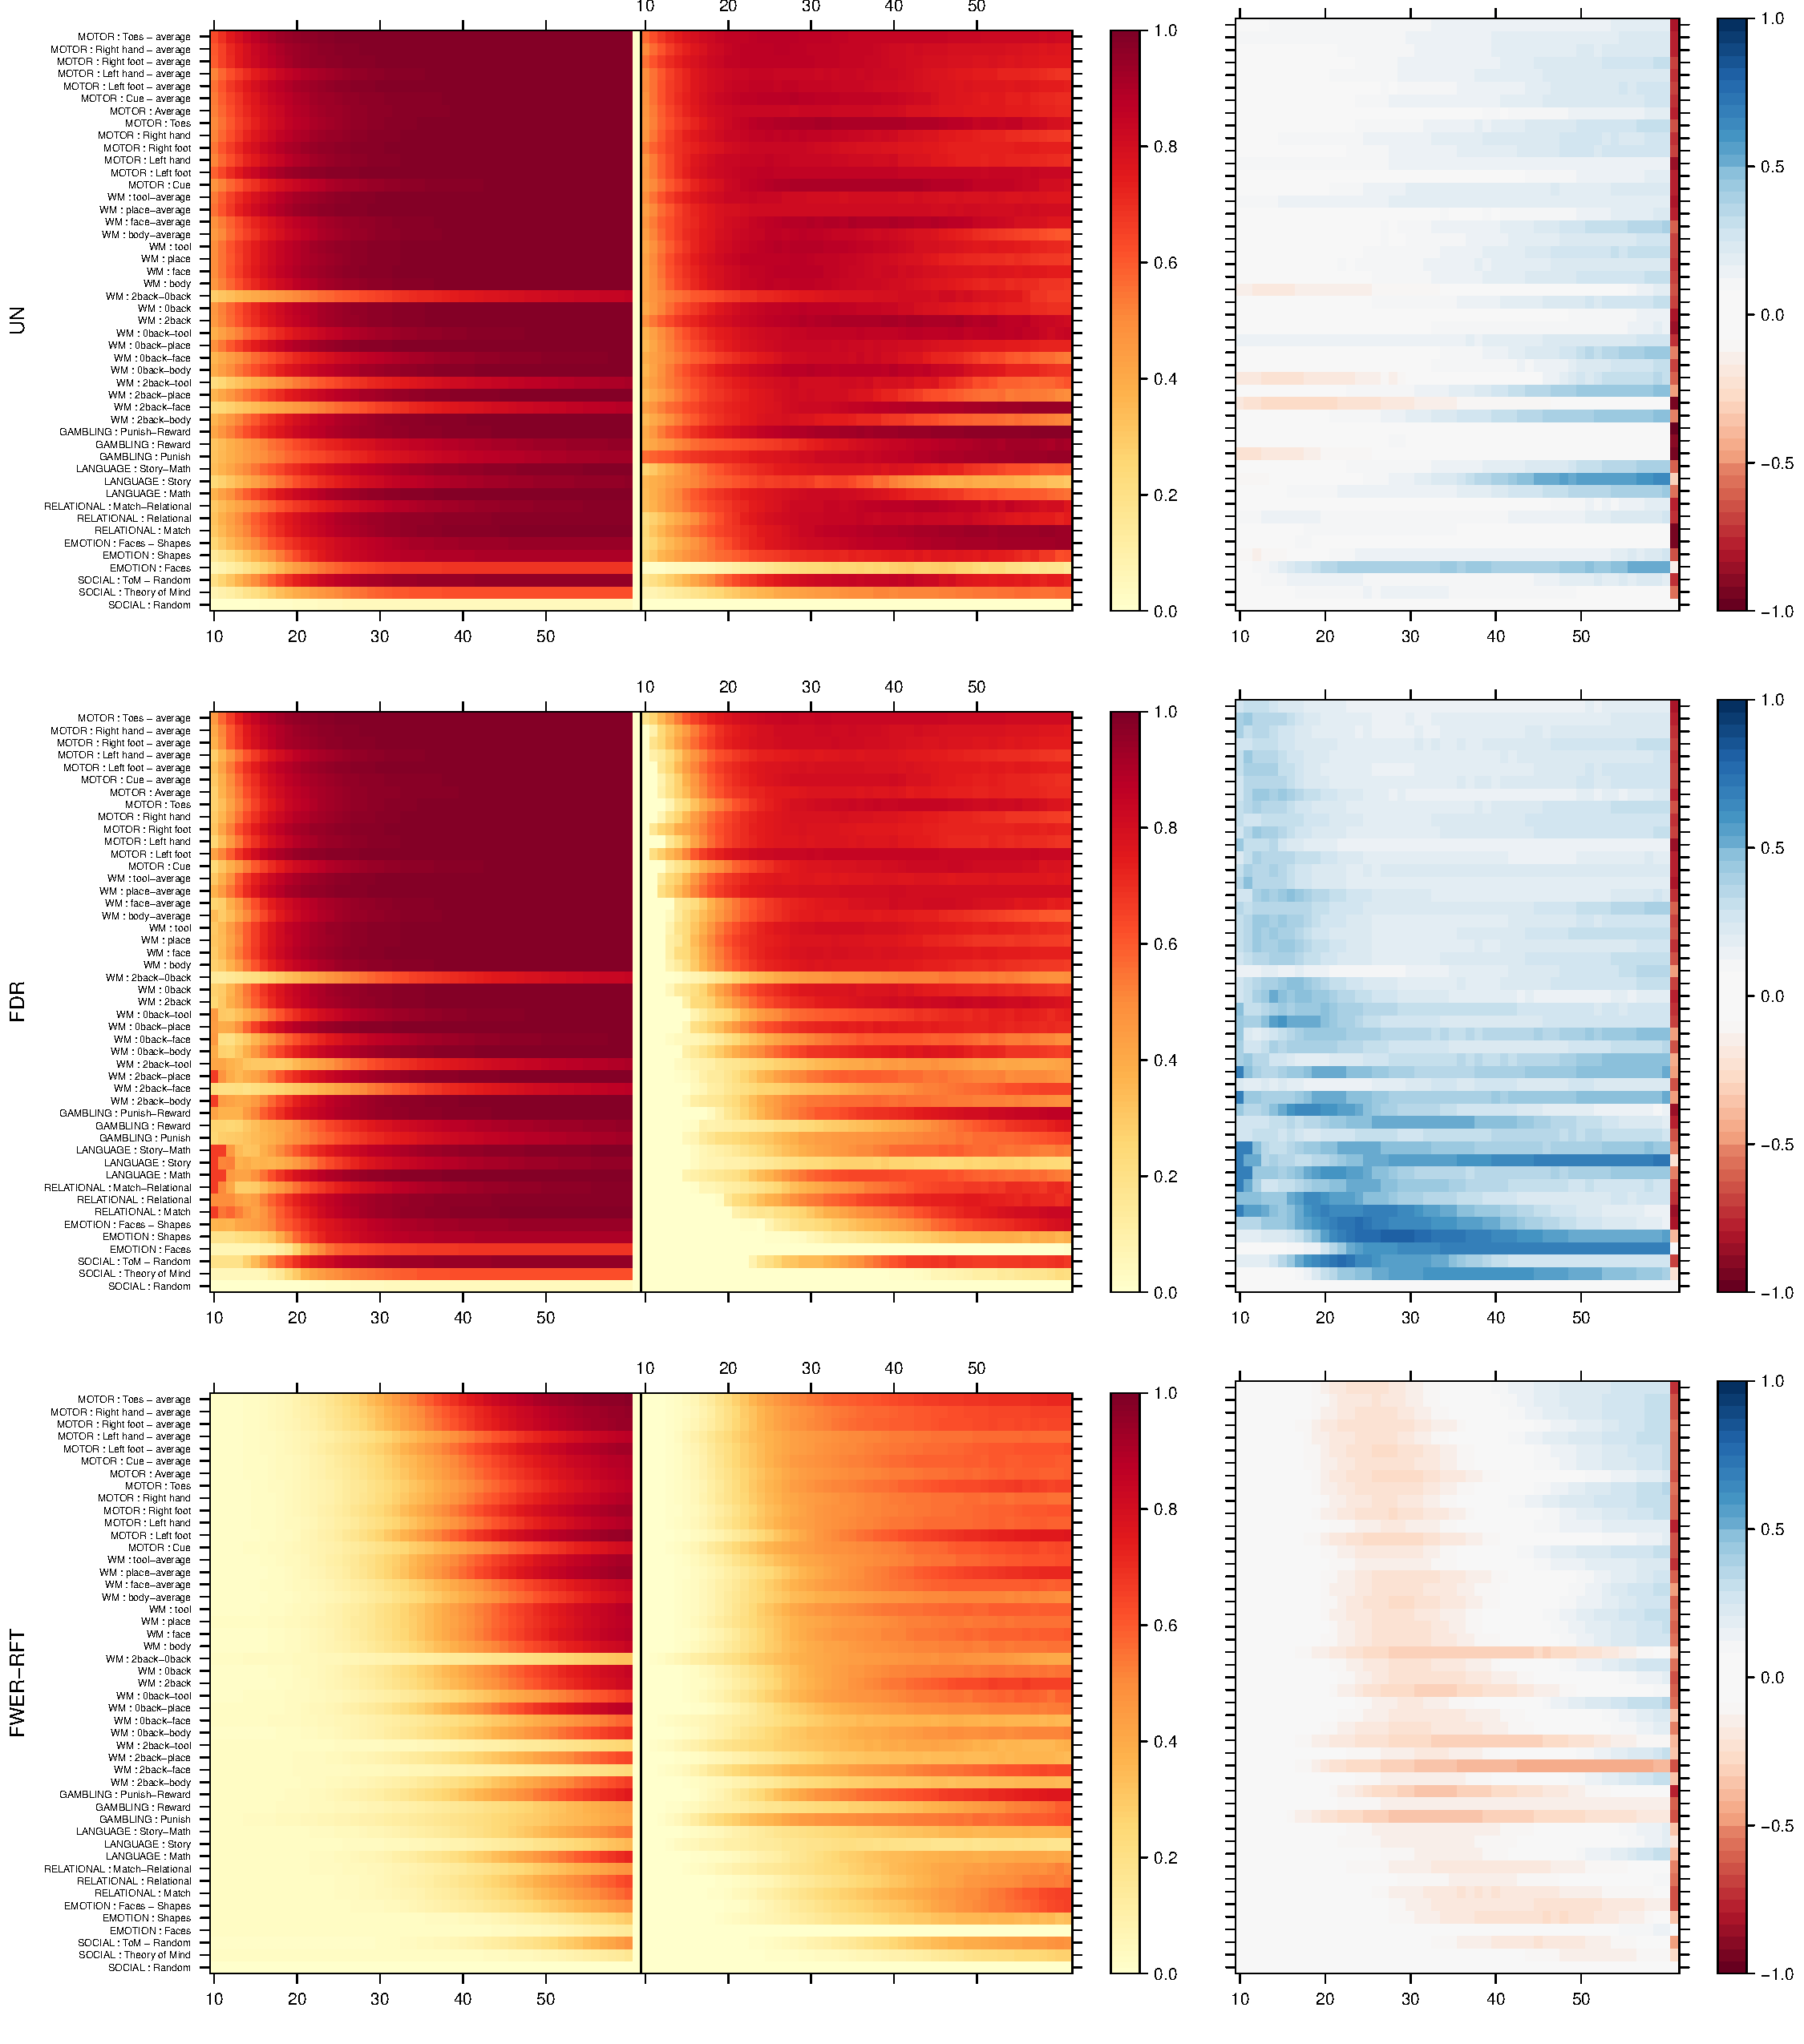
\includegraphics[scale=0.4]{FIG_HCP_10_power.pdf}
\caption{HCP results.  Evaluation of the power estimation over different subjects for all unique HCP-contrasts for thresholding with different error rate corrections at $\alpha=0.05$ from a pilot study with 10 subjects. The left column shows the estimated power curves, the middle column shows the true power and the right column shows the bias.  Bias is defined as the estimated power minus the true power.  The contrasts are sorted by their average empirically derived effect size. \label{SIM_pow_10}}
\end{figure}
\end{center}

\clearpage
